\documentclass[a4paper,french,bookmarks,12pt]{article}

\usepackage[
    top             = 0.6in,
    bottom          = 0.6in,
    inner           = 0.8in,
    outer           = 1.2in,    
    headheight      = 0.1in,
    headsep         = 0.4in,
    footskip        = 0.4in,
    marginparwidth  = 0.0in,
    marginparsep    = 0.0in,
    includeheadfoot, heightrounded, twoside
    ]{geometry}
\usepackage{Library}
\usepackage{caption}
\usepackage{pdflscape}
\usepackage{sidenotes}
\usepackage[skip=6pt plus1pt,indent=32pt]{parskip}
\usepackage{listings}
\usepackage{svg}
\usepackage{pdfpages}
\usepackage{booktabs}

\definecolor{pure-red}{HTML}{FF0000}
\definecolor{pure-green}{HTML}{00FF00}
\definecolor{pure-blue}{HTML}{0000FF}

\setlength\heavyrulewidth{0.35ex}

\DeclareCaptionLabelSeparator{figuresep}{}

\DeclareCaptionLabelFormat{figureformat}{%
    \colorbox{ensae!10}{\textnormal{\color{ensae}\sffamily\bfseries \,#1 #2\,}}
}

%\captionsetup[figure]{font=figurefont}
%\captionsetup[figure]{labelfont={bf},labelformat={default}}
\DeclareCaptionFont{figuretext}{\itshape}
\captionsetup[figure]{labelformat=figureformat,font=figuretext,labelsep=figuresep}
\captionsetup[table]{labelformat=figureformat,font=figuretext,labelsep=figuresep}

\captionsetup[sidenotes]{labelformat=figureformat,font=figuretext,labelsep=figuresep}

\DeclareCaptionStyle{widefigure}{options=sidenotes}
\DeclareCaptionStyle{marginfigure}{options=sidenotes}

\titlespacing*{\section}
{0pt}{5.5ex plus 1ex minus .2ex}{4.3ex plus .2ex}
\titlespacing*{\subsection}
{0pt}{5.5ex plus 1ex minus .2ex}{4.3ex plus .2ex}
%\renewcommand{\baselinestretch}{1.1}


\usepackage{tocloft}
\cftsetindents{section}{0em}{2.5em}
\cftsetindents{subsection}{2.5em}{3em}

\usepackage[backend=biber,style=apa,language=auto,
            autolang=langname]{biblatex}
\appto{\bibsetup}{\sloppy}
\addbibresource{bibliography.bib}


\makeatletter
\renewcommand\tableofcontents{%
    \@starttoc{toc}%
}

\renewcommand*\l@subsection{\@dottedtocline{2}{2em}{3em}}

\RenewDocumentCommand\sidenotetext{ o o +m }{%      
    \IfNoValueOrEmptyTF{#1}{%
        \@sidenotes@placemarginal{#2}{\textsuperscript{\thesidenote}{}~\footnotesize#3}%
        \refstepcounter{sidenote}%
    }{%
        \@sidenotes@placemarginal{#2}{\textsuperscript{#1}~#3}%
    }%
}
\ExplSyntaxOn
\NewDocumentEnvironment{widetext}{}{\begin{autoadjustwidth}{}{-\@sidenotes@extrawidth}}{\end{autoadjustwidth}}
\NewDocumentEnvironment{widetextl}{}{\begin{autoadjustwidth}{-\@sidenotes@extrawidth}{}}{\end{autoadjustwidth}}
\ExplSyntaxOff
\makeatother

\newcommand{\mkbibbracketscol}[1]{\textcolor{ensae}{\mkbibbrackets{#1}}}
\DeclareCiteCommand{\parencite}[\mkbibbracketscol]
  {\usebibmacro{prenote}}
  {\usebibmacro{citeindex}%
   \usebibmacro{cite}}
  {\multicitedelim}
  {\usebibmacro{postnote}}

\renewcommand{\thesection}{\Roman{section}}



\begin{document}  
    \title{Réduction de l’incertitude en segmentation médicale par méthodes d’ensemble}
    \author{SIAHAAN--GENSOLLEN Rémy}
    \date{\today}
    \hypersetup{
        pdftitle={Réduction de l’incertitude en segmentation médicale par méthodes d’ensemble},
        pdfauthor={SIAHAAN--GENSOLLEN Rémy},
        pdflang={fr-FR},
        pdfsubject={Réduction de l'incertitude en segmentation médicale par méthodes d'ensemble},
        pdfkeywords={medical segmentation, artificial intelligence, uncertainty}
    }
    
    \fancypagestyle{plain}{
        \fancyhf{}
        \renewcommand{\headrulewidth}{0pt}
        \renewcommand{\footrulewidth}{0pt}
        \fancyfoot[RO,LE]{\sffamily\color{white5}\thepage}
        \fancyhead[LE]{\sffamily\color{white5}Réduction de l’incertitude en segmentation médicale par méthodes d’ensemble}
        \fancyhead[RO]{\sffamily\color{white5}\nouppercase\leftmark}
    }
    
    \pagestyle{empty}
    \pagenumbering{gobble}
    \includepdf[]{cover statapp.pdf}
    
    \cleardoublepage

    \pagenumbering{arabic}\pagestyle{plain}
    \begin{tcolorbox}[
        enhanced,
        frame hidden,
        sharp corners,
        interior style = {color = ensae},
        spread upwards      = 0.1in,
        top                 = 0.6in, 
        bottom              = 0.4in
    ]
        \centering\color{white}\vspace{-0.2in}
        {\small{Rapport de projet de statistique et science des données appliquées}}        \vspace{0.2in}

         \textsc{Cumunel} Lucas, \textsc{Leroux} Tara, \textsc{LEROY} Léo, \textsc{Siahaan--Gensollen} Rémy\\
         \normalsize{\emph{Supervisé par : }} \large{\textsc{Coubez} Xavier PhD, \textsc{Kirscher} Tristan}
        
        \vspace{0.3in}\raisebox{-0.5mm}{\scalebox{3}{---}}
        
        \vspace{0in}\sffamily
        %\LARGE Segmentation médicale : gérer l'incertitude et la variabilité inter-experts
        \Large{Réduction de l'incertitude en segmentation médicale par méthodes d'ensemble}
    \end{tcolorbox}

    \medskip

    \begin{center}\sffamily\textbf{RÉSUMÉ}\end{center}
    %
    \medskip
    %
    La segmentation automatique des organes, bien que très utile en imagerie médicale, reste sujette à une forte incertitude, notamment lorsqu’elle repose sur des annotations manuelles potentiellement subjectives. Ce projet présente une évaluation systématique de méthodes d’ensemble de réseaux U-Net pour réduire cette incertitude. Nous entraînons et inférons plusieurs modèles sur des scans tomodensitométriques de patients annotés par différents experts, que nous combinons à l’aide d’une méthode d’ensemble. Ensuite, nous proposons et appliquons à ces prédictions un cadre d’évaluation systématique de leur précision, de leur incertitude aléatoire et de leur incertitude épistémique. Nos résultats indiquent que les méthodes d’ensemble utilisées diminuent significativement les incertitudes des prédictions sans détériorer leur précision.
    %
    \medskip

    \makeatletter
    \renewcommand\tableofcontents{%
        \@starttoc{toc}%
    }
    \makeatother

    \begin{tcolorbox}[
        enhanced,
        frame hidden,
        sharp corners,
        detach title,
        halign=left,
        spread outwards,
        halign              = center,
            valign              = center,
        borderline west     = {3pt}{0pt}{ensae},
        coltitle            = ensae, 
        interior style      = {
            color      = main1white2!65!gray!11
        },
        arc                 = 0 cm,
        title               = SOMMAIRE,
        boxrule             = 0pt,
        fonttitle           = \bfseries\sffamily,
        overlay             = {
            \node[rotate=90, minimum width=1cm, anchor=south,yshift=-0.8cm]
            at (frame.west) {\tcbtitle};
        },
    ]
        \begin{minipage}[t]{0.85\linewidth}
            \scriptsize\sffamily
            \tableofcontents
        \end{minipage}
    \end{tcolorbox}

    \newpage
    \section{Contexte et projet}

    \subsection{Introduction}

    \begin{widetext}
        \begin{minipage}{0.4\linewidth}
            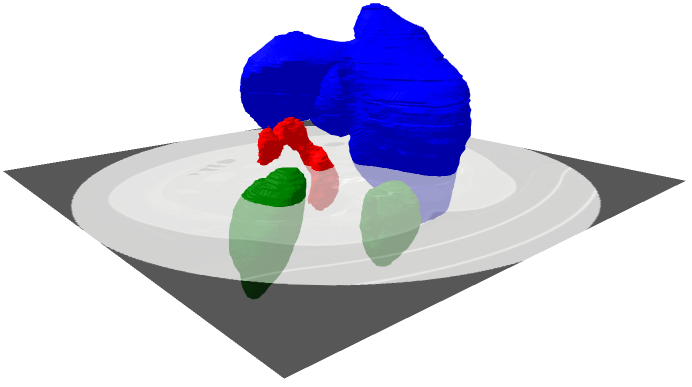
\includegraphics[width=1\textwidth]{figure_UKCHLL001_3D.png}
            \captionof{figure}{Segmentation 3D du {\color{ensae}pancréas}, des {\color{pure-green}reins} et du {\color{pure-blue}foie} d'un patient, ainsi qu'une coupe du scanner abdominal utilisée pour les délimiter.}
            \label{figure:3d}
        \end{minipage}
        %
        \hfill
        %
        \begin{minipage}{0.57\linewidth}
            \hspace{32pt} L'intelligence artificielle transforme la pratique médicale depuis plusieurs années, aidant les médecins à poser des diagnostics et à guider leurs décisions. L'imagerie médicale, joue un rôle central dans la prise en charge des patients \parencite{medicalimage}. La segmentation automatique --- c'est-à-dire la délimitation précise des organes et des structures par des algorithmes --- facilite le diagnostic, la planification du traitement et le suivi clinique. On retrouve parmi ces algorithmes les  réseaux de neurones convolutifs (\emph{Convolutional Neural Network}, ou \emph{CNN}), puissant outil d’apprentissage profond (\emph{deep learning}) ayant surpassés les experts humains dans de nombreuses tâches de compréhension d'images \parencite{Sarvamangala2022}. Particulièrement, une architecture de CNN très utilisée pour la segmentation médicale est le réseau U-Net \parencite{unet}.
        \end{minipage}
    \end{widetext}

    Cependant, beaucoup des structures et anomalies analysées (organes, vaisseaux sanguins, tumeurs, etc.) sont particulièrement complexes et variables, conduisant à une certaine \emph{incertitude} dans leur délimitation. Cette incertitude est accentuée par la \emph{variabilité inter-experts} : différents spécialistes médicaux peuvent avoir des opinions divergentes sur l'emplacement précis des limites des entités segmentées. Elle s'accroît d'autant plus lorsque plusieurs structures sont prédites simultanément (\emph{problème multi-classes}). Les réseaux de neurones doivent composer avec ces divergences, conduisant parfois à des incohérences dans les résultats de segmentation, ce qui peut directement impacter les décisions médicales, et donc le patient). 
    
    Quantifier ces incertitudes permet de générer des cartes d'incertitude sur les images médicales pour isoler les zones où les médecins doivent redoubler d'attention, fournir aux cliniciens des prédictions mieux calibrées et intégrer des mesures de confiance dans la prise de décision \parencite{values}. Cela améliore non seulement la sécurité des diagnostics assistés par IA, mais rend également les algorithmes plus transparents et fiables pour les applications médicales. Quantifier les incertitudes permet également d'évaluer l'impact des choix de méthodologie pour l’apprentissage machine : architectures des réseaux, tailles des jeux de données, durée d'entraînement, etc\dots{} Les méthodes d’apprentissage d'ensemble, qui consistent à combiner plusieurs modèles individuels ou leurs prédictions, sont un choix courant pour améliorer la performance des modèles d'intelligence artificielle \parencite{Ganaie_2022}. 

    Ce projet de statistiques appliquées consiste à évaluer l'impact sur l'incertitude de méthodes d'ensemble de modèles de segmentation médicale automatique. La sous-section suivante donnera une présentation de la quantification de l'incertitude et de son état de l'art. Les sections suivantes détaillerons l'expérience, la méthodologie d'évaluation, et discuterons des résultats obtenus.

    \subsection{Quantification de l'incertitude}

    Pour les médecins, connaître la fiabilité d'une segmentation est essentiel. Cependant, les modèles d’apprentissage machine n'indiquent pas systématiquement clairement leur niveau de confiance dans les prédictions qu'ils font : c'est le problème de \emph{l'incertitude dans les prédictions algorithmiques}. Par ailleurs, les experts médicaux peuvent annoter la même image différemment en raison de l'ambiguïté de certaines structures anatomiques. Ces désaccords réduisent la qualité des annotations utilisées pour entraîner les modèles et compliquent l'évaluation de leurs performances.     Nous présentons ci-dessous, dans La figure~\ref{figure:contour9}, trois coupes du scan tomodensitométrique (qu'on désignera aussi dans ce rapport par scan abdominal, ou de \emph{CT scan}, sans distinctions) du premier patient du jeu de données fourni pour le défi \text{CURVAS} (plus de détails plus tard), ainsi que les trois annotations du pancréas, du rein et du foie. La figure~\ref{figure:disagree} met en évidence les zones de désaccord :
    %
    \begin{widetext}
        \begin{minipage}{0.485\linewidth}
            \centering
            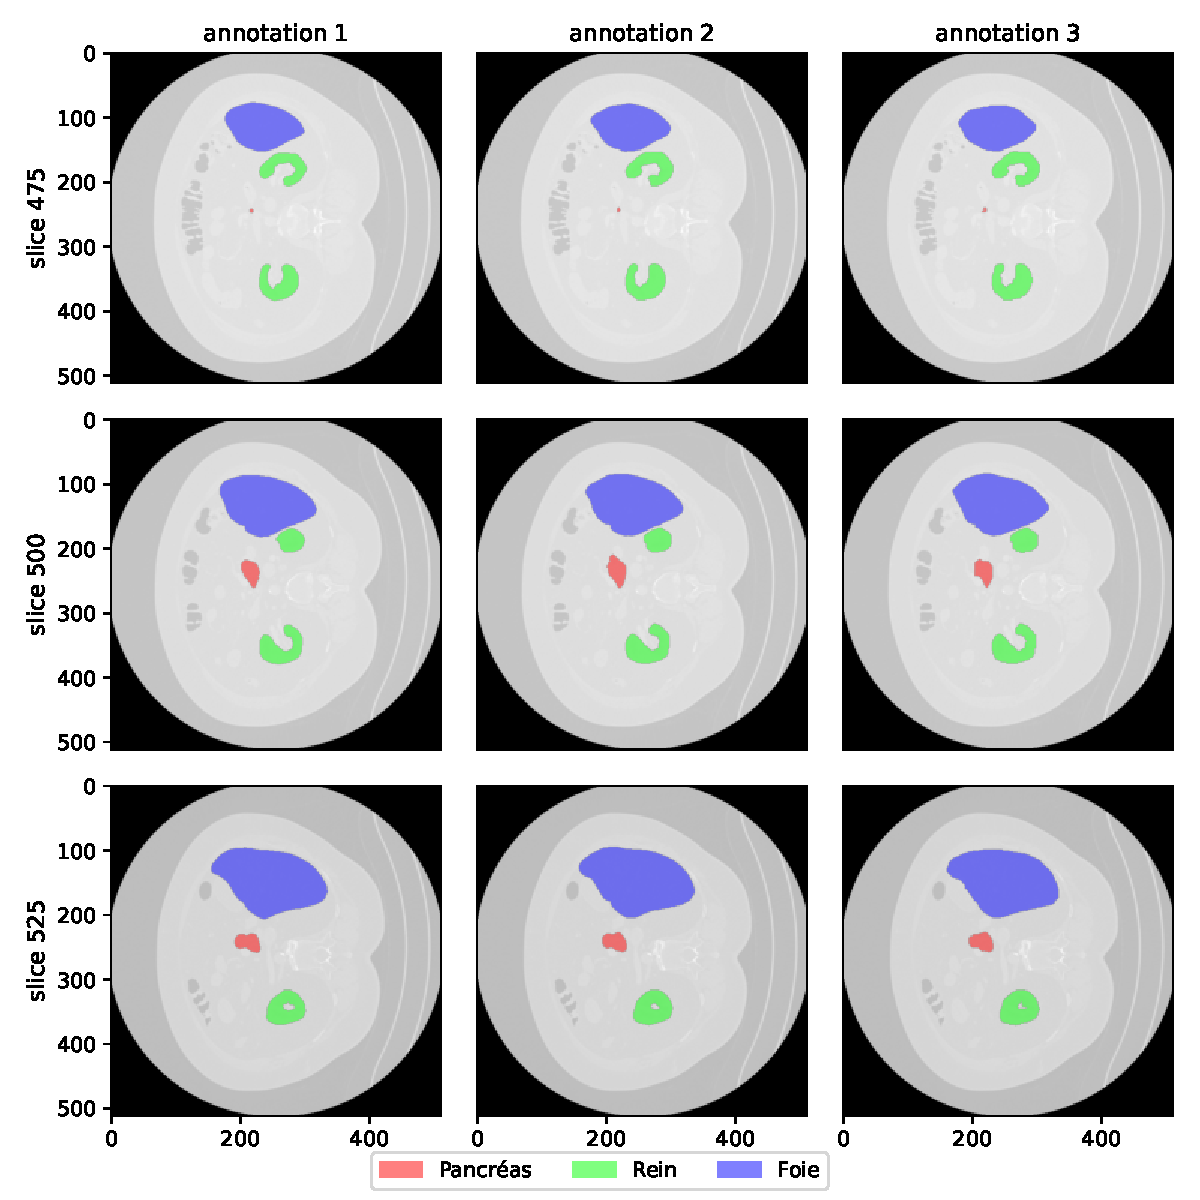
\includegraphics[width=\linewidth]{figure_UKCHLL001.pdf}
            \captionof{figure}{Contours réalisés par trois médecins pour différents organes sur trois coupes de CT scan sur le même patient.}
            \label{figure:contour9}
        \end{minipage}
        %
        \hfill
        %
        \begin{minipage}{0.485\linewidth}
            \centering
            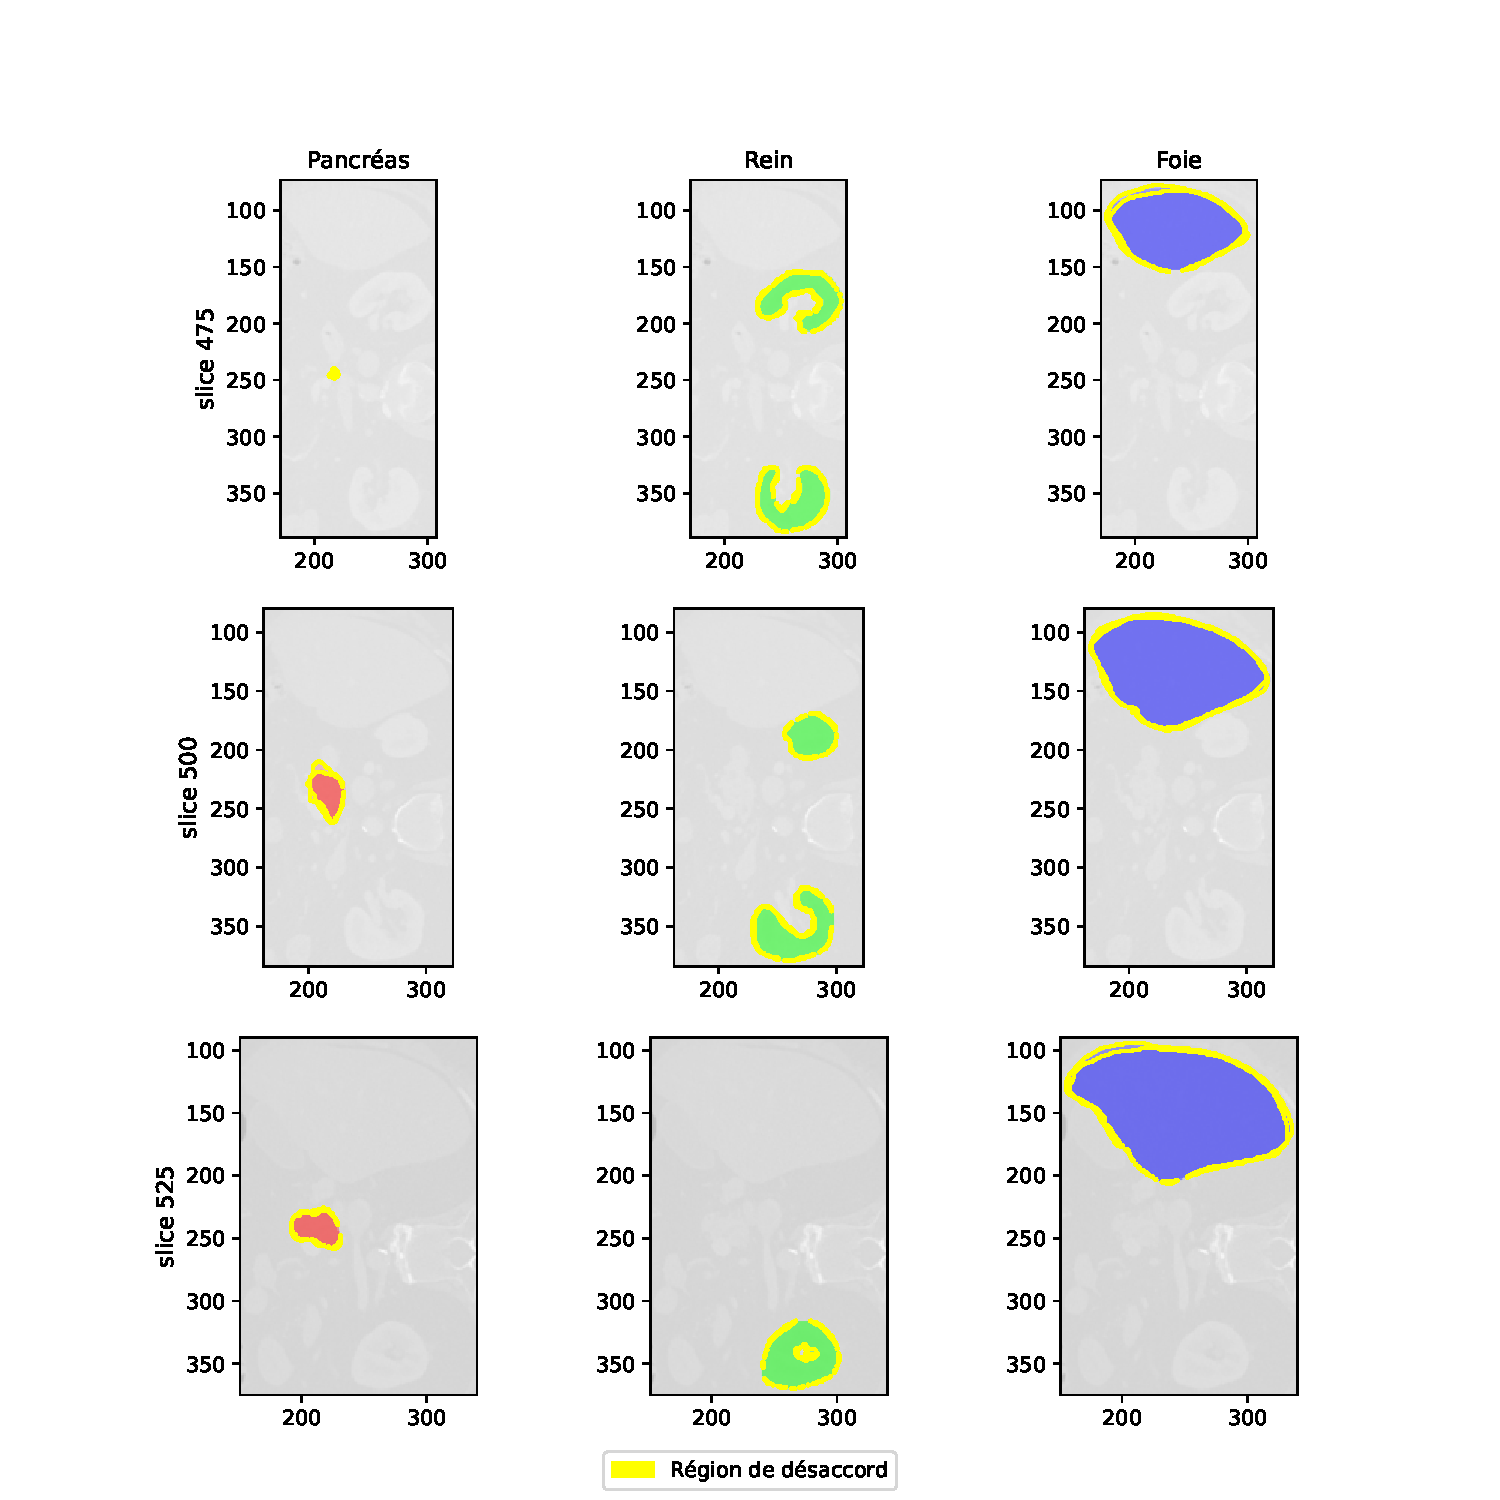
\includegraphics[width=\linewidth]{figure_UKCHLL001_disagree_region.pdf}
            \captionof{figure}{Zones de dissensus, mises en évidence en jaune}
            \label{figure:disagree}
        \end{minipage}
    \end{widetext}
    %
    \medskip
    %
    Théoriquement, nous pouvons distinguer deux types d'incertitude, qui combinés donnent l'incertitude prédictive (\emph{Predictive Uncertainty}, ou \emph{PU}) :
    %
    \begin{itemize}
        \item L'incertitude aléatoire (\emph{Aleatoric Uncertainty}, ou \emph{AU}) qui provient des données et est liée aux ambiguïtés inhérentes à l'image. On peut citer comme cause d'incertitude aléatoire les artefacts, les erreurs de numérisation, etc\dots{} Entre autres, l'exemple ci-dessus des désaccords entre annotateurs rentre dans cette catégorie.
        \item L'incertitude épistémique (\emph{Epistemic Uncertainty}, ou \emph{EU}), qui provient du modèle d’apprentissage lui-même. On peut citer comme cause d'incertitude épistémique un manque de connaissances (pas assez de données diversifiées observées durant l'entraînement), une architecture ne permettant pas de bien les \guill{apprendre}, etc\dots
    \end{itemize}
    %
    L'approche la plus notable pour capturer ces incertitudes a été introduite par \parencite{kendall2017}, qui l'envisagent du point de vue d'un classificateur bayésien. Ce classificateur reçoit une entrée \( x \) et produit des probabilités pour les classes $Y$ : 
    %
    \[ \bbP\p{Y \enstq x} = \bdE_{\omega \sim \Omega}\intc{\bbP\p{Y \enstq x, \omega}} \]
    %
    où les paramètres du modèle $\Omega$ suivent $\bbP\p{\omega \enstq D }$ pour les données d'entraînement $D$. 
    
    Ce cadre bayésien \parencite{smerkous2024} suppose que l'incertitude épistémique est représentée par l'entropie prédictive (\emph{Predictive Entropy}, ou \emph{PE}), qui est la somme de l'information mutuelle (\emph{Mutual Information}, ou \emph{MI}) et de l'entropie attendue (\emph{Expected Entropy}, ou \emph{EE}) représentant respectivement l'incertitude épistémique et l'incertitude aléatoire. En notant $\bbH$ l'entropie de \textsc{Shannon}, on a :
    %
    \[
    \underbrace{\bbH\p{Y \enstq x}}_{PU = PE} = \underbrace{\text{MI}(Y, \Omega|x)}_{EU = MI} + \underbrace{\mathbb{E}_{\omega \sim \Omega}[H(Y|\omega, x)]}_{AU = EE \ \text{(pour x i.i.d.)}}
    \]
    %

        La figure~\ref{fig:uncertainty} illustre les deux types d'incertitudes pour une régression unidimensionnelle : 
    %
    \begin{widetext}    
        \begin{minipage}{0.45\linewidth}
            \begin{tikzpicture}
              \begin{axis}[
                width=\linewidth,
                height=5.7cm,
                xmin=-15, xmax=15,
                ymin=0,   ymax=170,       % axe y de 0 à 170
                xlabel={$x$},
                ylabel={$g(x)$},
                axis on top,
                axis lines=left,
                ticks=none,
                axis line style={
                  line width=1pt,
                  -{Stealth[length=6pt,width=6pt]}
                },
                clip=true,               % clip réactivé
              ]
            
                % arrière-plan coloré (y de 0 à 170)
                \addplot [ensae!20,  fill=ensae!20,  draw=none]
                  coordinates {(-15,0) (-15,170) (-10,170) (-10,0)} \closedcycle;
                \addplot [pure-green!20, fill=pure-green!20, draw=none]
                  coordinates {(-10,0) (-10,170)  (-5,170)  (-5,0)}  \closedcycle;
                \addplot [white!20,      fill=white!20,      draw=none]
                  coordinates {(-5,0)   (-5,170)   (5,170)   (5,0)}   \closedcycle;
                \addplot [pure-blue!20,      fill=pure-blue!20,      draw=none]
                  coordinates {(5,0)    (5,170)    (10,170)  (10,0)}  \closedcycle;
                \addplot [ensae!20,  fill=ensae!20,  draw=none]
                  coordinates {(10,0)   (10,170)   (15,170)  (15,0)} \closedcycle;
            
                % fonction vraie g(x)=x^2+2x+3 décalée de +10
                \addplot [domain=-15:15, samples=200, ensae, thick] {x^2 + 2*x + 3 + 10};
            
                % points d'entraînement y+10
                \addplot [only marks, mark=*, black, mark size=1pt] coordinates {
                  % région [-10,-5]
                  (-7.256,54.125) (-6.424,41.010) (-6.986,48.461) (-7.276,49.675)
                  (-7.882,54.252) (-6.771,46.606) (-7.812,60.133) (-5.541,31.138)
                  (-5.182,34.026) (-8.083,59.257) (-6.041,37.507) (-7.356,52.018)
                  (-7.160,53.008) (-5.372,34.053) (-9.645,87.043) (-9.564,86.104)
                  (-9.899,89.415) (-5.837,31.434) (-6.109,37.408) (-5.650,33.935)
                  % région [5,10]
                  (8.334,94.012)  (8.353,87.676)  (6.052,61.448)  (5.645,60.434)
                  (6.577,70.078)  (6.819,76.155)  (7.851,83.997)  (7.193,75.498)
                  (9.942,125.000) (5.510,50.787)  (6.044,53.492)  (5.807,41.066)
                  (8.266,99.625)  (6.266,60.784)  (7.332,65.113)  (6.222,68.787)
                  (5.795,49.097)  (5.552,55.447)  (8.282,105.440) (5.691,58.058)
                };
            
              \end{axis}
            \end{tikzpicture}
            \captionof{figure}{Illustration des incertitudes épistémiques et aléatoires pour une régression 1D.}
            \label{fig:uncertainty}
        \end{minipage}
        %
        \hfill
        %
        \begin{minipage}{0.52\linewidth}
            %
            \begin{itemize}
                \item dans les régions rouge, on a une forte incertitude épistémique car le modèle n'a jamais vu de données dans ces plages et a pourtant fourni une approximation ; 
                \item dans la région blanche, on a seulement quelques points de données, donc une incertitude épistémique modérée ; 
                \item dans la région verte, on a peu de variance donc une incertitude aléatoire faible ; 
                \item dans la région bleue, enfin, on a plus de variance donc une incertitude aléatoire plus importante.
            \end{itemize}
        \end{minipage}
    \end{widetext}
    %
    \medskip
    
    Un autre concept très important est celui de \emph{calibration}. Les réseaux de neurones produisent des distributions de probabilités sur les étiquettes de classe possibles, ce qui fournit une mesure naturelle de l'incertitude. Idéalement, un modèle bien calibré devrait avoir une confiance élevée pour les prédictions correctes et une faible confiance pour les prédictions incorrectes. Cependant, les architectures modernes échouent souvent à atteindre cette calibration parfaite. Pour évaluer la calibration, des diagrammes de fiabilité (ou graphiques de calibration) sont utilisés. Ces graphiques comparent la confiance prédite avec la précision réelle, mettant en évidence les écarts (écarts de calibration). La figure~\ref{fig:calibration} illustre trois cas :
    %
    \begin{widetext}    
        \begin{minipage}{0.45\linewidth}
            \begin{tikzpicture}
              \begin{axis}[
                width=\linewidth,
                height=5.7cm,
                xmin=0, xmax=1, ymin=0, ymax=1,
                axis lines=left,
                ticks=none,
                axis line style={
                  line width=1pt,
                  -{Stealth[length=6pt,width=6pt]}
                },
                xlabel={Confiance},
                ylabel={Précision},
                xlabel style={at={(axis description cs:0.5,-0.05)},anchor=north},
                ylabel style={at={(axis description cs:-0.05,0.5)},anchor=south},
              ]
                % calibration parfaite
                \addplot [domain=0:1, samples=2, black, densely dotted, line width=1pt] {x};
                % sous-confiance (steeper)
                \addplot [domain=0:1, samples=2, blue, thick] {1.2*x};
                % sur-confiance (flatter)
                \addplot [domain=0:1, samples=2, red, thick]  {0.8*x};
              \end{axis}
            \end{tikzpicture}
            \captionof{figure}{Illustration des calibrations}
            \label{fig:calibration}
        \end{minipage}
        %
        \hfill
        %
        \begin{minipage}{0.52\linewidth}
            %
            \begin{itemize}
                \item calibration parfaite (ligne en pointillés noirs), où la précision correspond à la confiance ;
                \item sous-confiance (ligne bleue), où le modèle est trop prudent (la précision dépasse la confiance) ;
                \item sur-confiance (ligne rouge), où le modèle est trop confiant (la confiance dépasse la précision).
            \end{itemize}
        \end{minipage}
    \end{widetext}
    %
    Mathématiquement, un modèle parfaitement calibré satisfait :
    %
    \[ \forall p \in \intc{0, 1},\qquad \bbP\p{\hat{Y} = Y \enstq \hat{P} = p} = p \]
    %
    Autrement, cela signifie que si le modèle attribue une probabilité de 80\% à une prédiction, il devrait avoir raison 80\% du temps.

    \section{Expérience}

    \subsection{Données et modèles}

    Tenu de mai à octobre 2024, le challenge \textsc{CURVAS} (\emph{Calibration and Uncertainty for Multi-Rater Volume Assessment in Multiorgan Segmentation}) mettait des équipes au défi de produire un modèle de segmentation précis déterminer la meilleure calibration et quantification de la variabilité inter-expert. Nous utilisons pour ce projet le jeu de données mis à disposition à l'occasion de ce challenge, contenant au total 90 CT scans de patients, chacun annoté par 3 experts différents pour délimiter le pancréas, les reins et le foie de chaque patient. Les figures~\ref{figure:3d}, \ref{figure:contour9} et \ref{figure:disagree} sont réalisées sur les données du premier patient de la cohorte. Ces scans tomodensitométriques ont été récupérés à l'University Hospital Erlangen entre août et octobre 2023. 20 CT scans ont été donnés pour l'entraînement (groupe A), 5 pour la validation (groupe A) et 65 pour le test (20 en groupe A, 22 en groupe B et 23 en groupe C).

    Pour les entraînements, nous avons utilisé le framework nnU-Net (no-new-UNet) \parencite{nnunet}, bibliothèque d'outil pour entraîner des réseaux U-Net de segmentation, et conçue spécifiquement pour la segmentation automatisée d'images biomédicales. Contrairement aux réseaux U-Net classiques \parencite{unet}, régulièrement utilisés pour la segmentation sémantique, nnU-Net configure automatiquement de nombreux paramètres en fonction des caractéristiques de l'ensemble de données. Ces configurations sont indispensables car, dans les hôpitaux, les images médicales sont produites avec différents instruments, ne respectant pas les mêmes conventions et ayant des formats différents (2D, 3D), différentes saturations, dimensions, \dots{} Toutefois, nnU-Net présente l'inconvénient d'être très coûteux en calculs et nécessite des GPU performants.

    Nous avons d'abord entraîné 9 modèles différents sur le jeu de données d’entraînement (20 patients) : pour chaque annotateur, nous avons entraînés trois modèles avec des initialisations différentes des poids, pour explorer des points différents de l'espace des pertes (\emph{loss landscape}). Par soucis de reproductibilité, les générateurs aléatoires des poids ont été déterminisées en fixant les graines (aussi appelées nombres aléatoires, ou \guill{seeds}) \texttt{112233}, \texttt{445566} et \texttt{778899}. Ensuite, nous avons inféré chacun de ces modèles sur le jeu de données de test (65 patients). Systématiquement, nous avons généré les probabilités (sorties softmax du modèle) pour chacun des modèles et des patients, que nous avons ensuite utilisés pour générer 4 ensembles : un pour chaque triplet de modèle pour le même annotateur, et un général sur l'ensemble des 9 modèles. Enfin, nous avons exécuté pour chacun des patients et les 13 modèles différents des calculs évaluant la précision des prédictions, les incertitudes aléatoires et épistémiques. Ces calculs et les résultats sont présentés dans les sections suivantes.

    \subsection{Outils et ressources}

    Tout d'abord, nous avons dû modifier la bibliothèque nnU-Net pour y intégrer les fonctionnalités dont nous avions besoin et qui n'étaient pas initialement présentes. La première a été l'arrêt anticipé/précoce (\emph{stop-early)} des l'entraînement, car celui-ci pouvait prendre plusieurs jours à finir même sans progrès notable. Nous avons donc limité la durée d'entraînement à 300 epochs (cycles d'entraînement) au plus, avec un arrêt anticipé lorsqu'il n'y avait pas d'amélioration notable pendant 20 epochs. Nous avons ensuite rajouté la possibilité de fixer des \guill{seeds} d'initialisation aléatoire mentionnée plus haut, également non présente dans la bibliothèque de base. Quand le réseau de neurones commence son entraînement, les poids des neurones sont dans un premier temps fixés aléatoirement selon un générateur de nombre aléatoire déterminisé par la \guill{seed} choisie, pour être ensuite ajustés pendant l'entraînement. Il est à noter que d'autres sources d'aléatoire peuvent intervenir --- notamment au sein du module \texttt{PyTorch} sur lequel repose nnU-Net, notamment du point de vue des algorithmes de descente de gradient et d'optimisation (ou \emph{optimizers})) --- néanmoins cette première déterminisation permettait de mieux fixer comment le loss landscape est exploré. 

    Les entraînements des modèles U-Net sur les scans tomodensitométriques en trois dimensions sont conséquents, même avec la fonctionalité d'arrêt anticipé. Ils nécessitent par ailleurs des cartes graphiques de calcul (GPU). Nous avons donc utilisés des instances disponibles sur les services Onyxia de l'\textsc{Insee} et du Groupe \textsc{Genes} auxquels nous avons eu accès. Même avec cela, les entraînements prenaient près d'une journée pour chacun des modèles.  Par ailleurs, plusieurs difficultés sont survenues pour l'inférence, la méthode d'ensemble et l'évaluation. En effet, les volumes de données transférés à chaque fois étaient particulièrement importants, et chaque instance étant limitée à 100 Go, nous avons du traiter individuellement chaque tâche et chaque patient (parfois même chaque modèle) sur des instances différentes.

    Du fait de cette décomposition importante de chaque tâche, nous avons dû faire très attention à la reproductibilité. Pour le stockage, l'\textsc{Insee} nous a généreusement mis à disposition un espace de stockage compatible avec le standard S3 d'Amazon (plus préceisément de la solution open source MinIO) pour le transfert de fichiers. Celui-ci contient actuellement plusieurs milliers de Go correspondant aux artefacts produits par nos entraînements. Nous avons alors développé une application interface en ligne de commande (\emph{Command-Line Interface}, ou \emph{CLI}) avec le module \texttt{Typer}, permettant d'interagir avec le stockage distant via une clé de service créée pour le projet, et partagée entre tous nos services. 
    
    
    Cette application avait sinon pour utilisation principale de permettre le lancement systématique de chaque tâche avec une granularité de contrôle maximale. Les figures \ref{fig:label1} et \ref{fig:label2} ci-dessous présentent respectivement les commandes de la CLI (voir également en annexe) et un exemple d'utilisation (inférence sur le patient 80 du troisième modèle de l'annotateur 2, montrant bien la granularité). Le développement de cet outil a été une des étapes les plus importantes du projet. Le code source contient près de 6 500 lignes de python et de documentation, écrites spécifiquement pour (voir annexe). Ce code est également disponible sur le dépôt GitHub du projet.
    
    %
    \begin{center}
        \includegraphics[width=\linewidth]{clihelp.png}
        \captionof{figure}{Liste des commandes de la CLI}
        \label{fig:label1}
    \end{center}
    %
    \bigskip
    %
    \begin{center}
        \includegraphics[width=\linewidth]{cli ex 2.png}
        \captionof{figure}{Exemple d'utilisation de la CLI pour l'inférence}
        \label{fig:label2}
    \end{center}

    Comme le code de calcul des métriques était trop lent, nous l'avons optimisé en utilisant le module \texttt{numba}. Celui-ci nous a permis d'optimiser les fonctions d'évaluation en les compilant à la volée en code machine, via le compilateur \texttt{llvm}. Ainsi, l'interprétation était effectuée non via le compilateur Python, mais à un niveau natif (comme du code C ou FORTRAN compilé), accélérant fortement les boucles et opérations numériques. Il est particulièrement efficace pour les traitements sur les tableaux, à condition d'utiliser des variables simples et statiquement typables. En l’occurrence, certains traitements voxel-à-voxel dans les images 3D médicales étaient après optimisation près de 100 fois plus rapides par rapport à l'interprétation python, et le temps total d'évaluation a été divisé par plus de 4.
    
    \subsection{Protocole expérimental détaillé}

    \subsubsection*{Téléversement des jeux de donnés}
    
    Dans un premier temps, nous avons récupéré les données du challenge \textsc{CURVAS} \parencite{curvas},  c'est-à-dire, obtenu et mis en ligne sur le S3 les scans de coupes transversales de l'abdomen de 90 patients ainsi que les annotations des 3 experts différents pour chacune d'elles. Ces annotations représentent les contours de trois organes : le pancréas, le rein et le foie. Tous ces fichiers sont au format \texttt{.nii.gz}, et contiennent des tenseurs de forme $\p{\text{organe}, X, Y, Z}$, pour $866$ tranches de $512$ par $512$ voxels de CT scans, avec une valeur du voxel en noir et blanc pour l'image et un entier entre $0$ et $4$ pour chaque annotation ($0$ représentant le fond, $1$ le pancréas, $2$ les reins et $3$ le foie).

    \subsubsection*{Entraînement}

    Ensuite, il a fallu entraîner le réseau de neurones nnU-Net sur 20 de ces patients. Pour ce faire, nous avons modifié le code d'nnU-Net qui fonctionne sur une base similaire à notre CLI, avec plusieurs commandes, pour appeler directement les fonctions nécessaires. Une fois ceci fait (notamment pour respecter la structure des dossiers et de l'enregistrement des fichiers d'entraînement, qui est fixée dans nnU-Net), nous avons donc tout d'abord téléchargé les données depuis le S3 puis lancé une étape de pré-traitement (\emph{preprocessing}) propre à nnU-Net, où des algorithmes étudient automatiquement chaque image pour normaliser les intensités lumineuses, les tailles, etc\dots. Cette étape étant la même pour chaque annotateur, notre CLI téléversait à la fin du preprocessing les fichiers générés sur le S3 pour ne pas avoir à relancer cette étape sur les entraînements ultérieurs. 
    
    Une fois les différents pré-traitements achevés, nous avons lancé les entraînements des 9 modèles. Par défaut, nnU-Net entraîne 5 \guill{folds} en validation croisée sur les 80 \% des données fournies. Manquant de ressources de calcul, nous avons exécuté un seul \guill{fold} sur l'ensemble des données fournies. Chacune des initialisations était déterminisée à l'aide d'une seed, en utilisant le code que nous avions implémenté. Nous avons fixé une limite à 300 epochs, avec un arrêt anticipé lorsque le DICE mesuré pendant l'entraînement ne s'améliorait pas sur 20 epochs. Les modèles entraînés étaient ensuite automatiquement transférés sur le stockage S3.

    nnU-Net génère automatiquement des fichiers checkpoint qui contiennent les poids du réseau de neurones à une étape donnée de l'entraînement. Nous utilisons ces fichiers pour l'inférence : à partir de ces poids et d'un nouveau CT scan, nous pouvons générer une nouvelle annotation. Ces fichiers sauvegardent des poids du réseau de neurones ce qui permet une reprise de l'entraînement en cas d'erreur ou de perte de connexion (arrêt du service). nnU-Net sauvegarde aussi automatiquement les poids offrant la meilleure performance. En effet, en raison de la descente de gradient stochastique, la performance peut diminuer légèrement lors de l'epoch suivante (période d'entraînement).  

    

    \subsubsection*{Inférence}

    Une fois les modèles entraînés, nous avons pu récupérer les prédictions des patients restants (64). L'inférence de nnU-Net demande tout d'abord de télécharger les modèles entraînés (donc depuis notre S3) et les scans abdominaux bruts. Comme nous devions de plus effectuer cette inférence sur 9 modèles, le tout représente 576 lancements et donc un temps de calcul très conséquent. L'inférence était particulièrement longue et surtout volumineuse du fait de la nécessité de produire les tenseurs des probabilités de sortie (c'est-à-dire pour chaque voxel, le softmax des logit --- score non normalisé --- associés aux trois classes d'organes et non simplement la classe prédite pour ce voxel, générée dans un fichier au format \texttt{.nii.gz}). Ces tenseurs avaient une dimension importante : (4, 866, 512, 512). Ces fichiers \texttt{.npz} faisaient donc tous plus de 3 Go. Une fois les prédictions effectuées, elles étaient également transférés automatiquement sur le S3.

    \subsubsection*{Méthodes d'ensemble}
    
    En utilisant les softmax générés à la phase d'inférence, nous avons pu prendre la moyenne des probabilités pour obtenir des prédictions correspondant aux différents ensemble. Cette phase téléchargeait donc pour chaque patient les 9 prédictions de la phase précédente (prédiction et softmax), et calculait de nouveaux softmax moyens pour les ensembles décrits plus haut (un par annotateur, et un global), puis générait les prédictions associées à ces modèles. Ainsi, en prenant la moyenne des prédictions, les ensembles sur même annotateur capturent une partie de l'incertitude épistémique, qui découle des limitations inhérentes du modèle à apprendre à partir des données disponibles. En moyennant sur plusieurs annotateurs, on peut également également capturer une partie de l'incertitude aléatoire. Les approches par méthodes d'ensembles sont particulièrement efficaces pour améliorer la robustesse et réduire la variance dans les tâches de segmentation \parencite{Ganaie_2022}. Une fois les softmax et prédictions calculées, elles sont automatiquement téléversées sur le S3.

    \subsubsection*{Préparation et récupération des métriques d'incertitude}

    Le but de ce projet étant de tester l'efficacité de nnU-Net et l'incertitude de sa segmentation avec un large panel de métriques, nous avons produit un fichier de calcul de ces métriques en les récupérant sur les dépôts de \textsc{CURVAS} et de \textsc{ValUES}. Le détail de ces métriques sera évoqué dans la partie suivante. De même que pour les étapes précédentes, pour chaque patient, nous avons téléchargé les prédictions (dont les softmax, nécessaires au calcul des métriques) avec les annotations des experts et appliqué notre jeu de métriques au 13 modèles, avant de transférer les données dans le S3 sous forme de \texttt{.csv}. Par ailleurs, nous avons dû mettre en place un système de parallélisation des calculs pour optimiser le temps d'exécution des métriques. Ainsi nous avons accéléré par plus d'un facteur quatre la durée d'exécution grâce au module \texttt{numba}.
    
    \subsubsection{Schéma résumé}

    La figure~\ref{fig:diagram} ci-dessous présente un résumé des différentes étapes. On traitera sinon plus qualitativement de ce dernier dans la section Discussion.
    %
    \medskip
    %
    \begin{center}
        \begin{tikzpicture}[
            box/.style={
              rectangle,
              fill=ensae!20,
              draw=none,
              align=center,
              minimum height=1.2cm,
              minimum width=6cm
            },
            arrow/.style={
              -{Stealth[length=5pt,width=5pt]},
              thick
            }
        ]
        
          % Données
          \node[box] (dtrain) {Jeu d'entraînement\\\emph{(20 patients)}};
          \node[box, right=of dtrain] (dtest) {Jeu de test\\\emph{(65 patients)}};
        
          % Entraînement
          \node[box, below=of dtrain] (train) {
            Entraînement de 9 modèles\\
            \emph{(3 seeds × 3 annotateurs)}
          };
        
          % Inférence
          \node[box, right=of train] (infer) {
            Inférence\\
            \emph{(prédictions et probabilités)}
          };
        
          % Ensembles
          \node[box, below=of train] (ens) {
            Construction des 4 ensembles\\
            \emph{(3 annotateurs et 1 général)}
          };
        
          % Évaluation
          \node[box, right=of ens] (eval) {
            Évaluation des modèles\\
            \emph{(métriques)}
          };
        
          % Connexions
          \draw[arrow] (dtrain) -- (train);
          \draw[arrow] (dtest)  -- (infer);
          \draw[arrow] (train)  -- (infer);
          \draw[arrow, bend right=8] (infer)  to (ens);
          \draw[arrow] (infer)  to (eval);
          \draw[arrow] (ens)    -- (eval);
          \draw[arrow, bend left=80] (dtest)  to (eval);
        \end{tikzpicture}
        \captionof{figure}{Diagramme résumant le protocole expérimental}
        \label{fig:diagram}
    \end{center}


    \section{Évaluation de l'incertitude}

    Cette section décrit de manière exhaustive le cadre d'analyse de la précision et de l'incertitude que nous avons utilisé pour évaluer les modèles et ensembles. Pour cela, nous avons recours à un panel de métriques issues du challenge \textsc{CURVAS} (Consensus-based DICE, Confidence, ECE, CRPS) \parencite{curvas} et du framework \textsc{ValUES} (ACE, AUROC, AURC, EAURC, NCC) \parencite{values}, ainsi que des mesures classiques de performance telles que l'entropie ou la distance de \textsc{Hausdorff}. Ces métriques permettent de capturer les deux types d'incertitudes, aléatoire et épistémique, ainsi que la performance globale des modèles.

    \subsection{Métriques de performance}

    Pour mesurer la performance des modèles, nous mesurons les écarts entre les annotations et les prédictions. Ces écarts sont obtenus selon les métriques suivantes : le consensus-based DICE, le CRPS, et la distance de \textsc{Hausdorff}.
    
    \subsubsection*{Consensus-based DICE}

    Le \emph{consensus-based DICE} est un DICE score ordinaire (mesure de la similitude entre deux espaces) mais prenant la zone de consensus (i~.e. tous les experts sont d'accord) et la prédiction. Cela permet de tenir compte des variabilités inter-experts (donc de l'incertitude aléatoire). Nous le calculons pour chaque organe et, comme un DICE classique, plus il s'approche de 1 plus la prédiction est correcte. Cette mesure nous permet d'avoir une idée générale de la performance du modèle en tenant compte de la variabilité inter-experts.
        
    \[ \text{DICE} = \frac{2 |P \cap G|}{|P| + |G|} \]
    
    \begin{itemize} 
        \item \( P \): Segmentation prédite.
        \item \( G \): Zone de consensus entre annotateurs.
        \item \( |P \cap G| \): Intersection entre les segmentations (i.e. voxels qui se recoupent).
        \item \( |X| \): Nombre total de voxel dans la segmentation X.    
    \end{itemize}
    

    \subsubsection*{CRPS (Continuous Ranked Probability Score)}
    
    Le \emph{Continuous Ranked Probability Score} estime la proximité entre le masque des annotations et le masque des probabilités prédites (une probabilité associée à chaque classe pour chaque voxel). Plus précisément il s'agit de la distance quadratique entre la fonction de répartition de la prédiction probabiliste et la fonction de répartition des annotations (qui est une fonction de Heaviside). Le CRPS, contrairement à la plupart des métriques, n'oscille pas entre 0 et 1 mais est un volume (somme des distances, mesurée en $mm^3$), que l'on souhaite le plus faible possible (faible écart entre annotations et prédiction). Comme le CRPS s'axe sur les probabilités prédites, il offre une perspective de perfomance complémentaire du DICE, d'où sa présence dans le challenge CURVAS et notre choix de le garder.
      
    \[ \text{CRPS}(F, x) = \int_{-\infty}^{\infty} \left( F(y) - \bdOne_{\{y \geq x\}} \right)^2 dy \]
    \begin{itemize}
        \item \( F(y) \): Fonction de répartition des probabilités prédites au point \( y \).
        \item \( \bdOne_{\{y \geq x\}} \): Fonction de répartition (ou de \textsc{Heaviside}) des annotations au seuil \(x\).
    \end{itemize}

    \subsubsection*{Distance de Hausdorff}

    La \emph{distance de \textsc{Haussdorff}} mesure l'écart le plus grand entre une annotation et une prédiction (soit la plus grande erreur de segmentation possible). Contrairement au DICE et au CRPS, nous la calculons pour chaque annotateur (pour tenir compte de la variabilité inter-expert). Bien qu'absente des évaluations de CURVAS et de ValUES, cette métrique nous paraissait importante car elle s'intéresse aux erreurs extrêmes de prédiction et est donc plus spécifique.

    \[ d_H(A, B) = \max\left\{ \sup\limits_{a \in A} \inf\limits_{b \in B} \|a - b\|, \sup_{b \in B} \inf_{a \in A} \|b - a\| \right\}
    \]
    \begin{itemize}
        \item \( A \): Segmentation prédite composée des valeurs des voxels \(a\).
        \item \( B \): Segmentation par un expert composée des valeurs des voxels \(b\).
    \end{itemize}

    \subsection{Métriques d'incertitude aléatoire}

    Comme expliquée plus haut, l'incertitude aléatoire elle est liée aux données d’entrée et notamment à l'ambiguïté des annotations humaines. Les autres sources possibles incluent donc les désaccords inter-annotateurs, le bruit ou les artefacts dans les images, ou des cas atypiques, pathologiques... Pour mesurer l'incertitude aléatoire ici, nous mesurons l'incertitude dans les annotations grâce à la Confiance  (ou Uncertainty Assessment) et la NCC.

    \subsubsection*{Confiance (ou Uncertainty Assessment)}

    L'\emph{Uncertainty Assessment} est justement une mesure de la confiance globale des annotations. C'est la moyenne de la confiance (consensus pour la classe) pour le \guill{Background} $C_B$ (éléments non pris en compte et le \guill{Foreground} $C_F$ (éléments d'intérêt, comme le pancréas ici). Ainsi, plus elle est haute, plus la confiance dans les annotations des experts est élevée. Cette métrique ne dépend pas d'un modèle (et de ses prédictions).
    %
    \[ C_{\text{seg}} = \frac{(1 - C_B) + C_F}{2} \]

    
    \subsubsection*{NCC (Normalised Cross Correlation)}

    La \emph{Normalised Cross Correlation} correspond, comme son nom l'indique, à une variante du coefficient de corrélation. Elle mesure donc, comme une corrélation, la similarité entre deux annotations de 0 à 1 en valeur absolue (1 indiquant une similarité parfaite), en utilisant leur carte d'incertitude (voir plus loin). Cette métrique permet de capturer la variabilité inter-expert par paires, permettant une plus grand précision que l'Uncertainty Assessment.
    %
    \[ \text{NCC}(A, B) = \frac{\sum (A - \bar{A})(B - \bar{B})}{\sqrt{\sum (A - \bar{A})^2 \sum (B - \bar{B})^2}} \]
    %
    \begin{itemize}
        \item \( A \): Carte d'incertitude d'une annotation.
        \item \( B \): Carte d'incertitude d'une autre annotation.
        \item \( \bar{X} \): Moyenne empirique des valeurs de X.
    \end{itemize}
    %
    \subsection{Métriques d'incertitude épistémique --- Calibration}

    Les métriques d'incertitude épistémique peuvent se décomposer en deux catégories. La première regroupe les métriques traitant des erreurs de \emph{calibration}, c'est-à-dire de décalage entre la confiance d'un modèle dans une prédiction et sa précision réelle. Elles estiment à quel point le modèle est fiable. La deuxième catégorie regroupe quant à elle les métriques traitant de la reconnaissance d'erreur, c'est-à-dire la quantification de la capacité du modèle à reconnaître les erreurs qu'il commet. Décrivons dans un premier temps les métriques de la première catégorie. Nous utilisons l'ECE --- proposée par \textsc{CURVAS} --- et l'ACE --- son pendant proposé par \textsc{ValUES} --- décrites plus bas. Si cette dernière a une méthode de calcul très similaire, elle permet une approche plus fine, notamment par le calcul des intervalles qui dépend de la distribution des probabilités prédites.
    
    \subsubsection*{ECE (Expected Calibration Error)}

    L'\emph{Expected Calibration Error} se calcule en séparant les probabilités prédites en plusieurs intervalles $B_m$, de 0 à 1 (appelés \emph{bins}). Puis, au sein de chaque \emph{bin}, on détermine la confiance et la précision moyenne. L'ECE est ainsi la somme pondérée (par la taille de l'intervalle) de la différence entre précision et confiance moyenne pour chaque (d'où le décalage évoqué au-dessus). L'ECE est une mesure phare de la calibration des modèles (elle est d'ailleurs l'unique mesure de calibration du challenge CURVAS et est même directement intégrée à la librairie \texttt{torchmetrics}, ce qui facilite son utilisation).
    %
    \[ \text{ECE} = \sum_{m=1}^{B} \frac{|B_m|}{n} \left| \text{acc}(B_m) - \text{conf}(B_m) \right| \]
    %
    \begin{itemize}
        \item \( B \): Nombre de bins.
        \item \( B_m \): Le \( m \)-ème bin.
        \item \( |B_m| \): Nombre de prédictions dans le bin  \( B_m \).
        \item \( n \): Nombre total de prédictions.
        \item \( \text{acc}(B_m) \): Précision (Proportion de prédictions correctes dans le bin \( B_m \)).
        \item \( \text{conf}(B_m) \): Confiance (moyenne des probabilités prédites dans le bin \( B_m \)).
        \item \( \frac{|B_m|}{n} \): Poids associés aux bins selon la proportion de prédictions qu'ils contiennent.
    \end{itemize}
    
    \subsubsection*{ACE (Average Calibration Error)}

    L'\emph{Average Calibration Error} est calculé de façon identique mais sans la pondération. Les bins sont déterminés de sorte à être de taille égale. ACE comme ECE se situent entre 0 et 1 avec une calibration qui peut être considérée comme correcte en-dessous des $0.1$ (ou même $0.05$). L'ACE permet un regard plus fin que l'ECE sur la calibration des modèles, notamment en isolant les potentiels effets de la distribution des probabilités prédites.
    %
    \[ \text{ACE} = \frac{1}{B} \sum_{b=1}^{B} \left| \text{acc}(b) - \text{conf}(b) \right| \]
    %
    \begin{itemize}
        \item \( B \): Nombre de bins \(b\) (de tailles égales).
        \item \( \text{acc}(B_m) \): Précision (Proportion de prédictions correctes dans le bin \( B_m \)).
        \item \( \text{conf}(B_m) \): Confiance (moyenne des probabilités prédites dans le bin \( B_m \)).
    \end{itemize}
    
    \subsection{Reconnaissance d'erreur (Failure Detection)}
    
    La reconnaissance d'erreur peut se mesurer à l'aide de métriques comme l'AUROC, l'AURC et l'EAURC.

    \subsubsection*{AUROC (Area Under the Receiver Operating Characteristic curve)}

    L'\emph{Area Under the Receiver Operating Characteristic curve} est une mesure de l'aire sous la courbe ROC (Taux de vrais positifs en fonction du taux de faux positifs). Plus précisément, cette courbe représente le rapport en vrais et faux positifs pour différents seuils (valeur à partir de laquelle on considère qu'une probabilité renvoie une valeur positive). Ainsi, une courbe ROC idéale serait dans le coin supérieur gauche d'un axe orthonormé (100 \% de vrais positifs et 0 \% de faux positifs) et donc son aire (AUROC) serait égale à 1. Cela signifie donc que le modèle distingue parfaitement les valeurs positives des négatives (absence d'organe). On voit ici l'intérêt de l'ajout du framework ValUES avec des métriques qui capturent d'autres causes de l'incertitude épistémique (en l'occurrence, liée à l'identification des erreurs).
    %
    \[ \text{AUROC} = \int_{0}^{1} \text{TPR}(t) \, d\text{FPR}(t) \]
    %
    \begin{itemize}
        \item \( \text{TPR}(t) \): Taux de vrais positifs au seuil \( t \).
        \item \( \text{FPR}(t) \): Taux de faux positifs au seuil \( t \).
    \end{itemize}

    \subsubsection*{AURC (Area Under the Risk Curve)}

    L'\emph{Area Under the Risk Curve} est aussi une aire mais d'une courbe de risque. Elle est tracée en prenant pour chaque probabilité prédite, le risque associé (ici, la différence entre annotation et prédiction). Chaque point correspond ainsi à un seuil de confiance (comme pour la ROC curve, on calcule le risque à différents seuils). Plus l'aire est faible, plus le risque est faible à chaque seuil et plus le modèle prédit avec une faible erreur. L'AURC complète l'AUROC en insistant sur l'arbitrage risque/qualité ; un autre apport bénéfique de ValUES.
        
        \[ \text{Risk}(t) = \frac{1}{N} \sum_{i=1}^{N} \left| y_i - \hat{y_i}(t) \right|,\qquad \text{AURC} = \int_{0}^{1} \text{Risk}(t) \, dt
        \]
        
\begin{itemize}

    \item \( y_i \): La valeur issue de l'annotation.
    \item \( \hat{y_i}(t) \): La valeur prédite au seuil \( t \).
    \item \( N \): Nombre de voxels de l'image.
\end{itemize}



        \vspace{0.2cm}
        \subsubsection*{EAURC (Expected Area Under the Risk Curve)}

        L'\emph{Expected Area Under the Risk Curve} est une version normalisée de l'AURC. Il s'agit de la différence entre l'AURC et l'AURC optimale (c'est-à-dire avec une répartition optimale des risques à chaque seuil). L'interprétation est sensiblement la même à cela près que l'EAURC est moins influencée par les erreurs récurrentes ou extrêmes.
        %
        \[ \text{EAURC} = \frac{1}{A^*} \int_{0}^{1} \text{Risk}(t) \,dt - \int_{0}^{1} \text{Risk}^{*}(t) \, dt \]
        %
        \begin{itemize}
            \item \( {A^*} \): Aire sous la courbe de risque optimale.
            \item \( \text{Risk}^*(t) \): Le risque optimal au seuil t.
        \end{itemize}
        
        \subsection{Entropie et cartes d'incertitudes}

        Comme on l'a mentionné en introduction, il est possible de générer des cartes d'incertitudes indiquant les points (ici les voxels) sur lesquels le modèle est le moins \guill{confiant} dans sa prédiction. Ici, on peut associer à chaque voxel $v$ un vecteur mesure de probabilité $p_v = \p{p_1, p_2, p_3, p_4}^\top$, tel que $p_1$ est la probabilité que ce voxel soit dans le fond, $p_1$ que ce soit le pancréas, $p_2$ les reins et $p_3$ le foie. Dans le cas où $p_1 = p_2 = p_3 = p_4 = 0,25$, la confiance est au plus bas (on ne peut distinguer une classe des autres). Dans le cas où $p_i = 1$ et $p_{j \neq i} = 0$, elle est au plus haut. On peut alors utiliser l'entropie pour caractériser cette confiance. L'\emph{entropie de Shannon} est une mesure assez générale de l'incertitude d'une segmentation. Elle l'établit en utilisant les probabilités prédites pour chaque classe des valeurs des voxels :
        %
        \[ \text{H}(p) = -\sum_{i} p_i \log p_i\]
        %
        \begin{itemize}
            \item \( p \): Vecteur de probabilités contenant les probabilités \(p_i\) associées à chaque classe.
        \end{itemize}
        %
        L'entropie peut être calculée à l'échelle de l'image, ou pour chaque voxel, ce qui permet notamment de générer des cartes d'incertitudes comme en figure~\ref{fig:uncertaintymap} ci-dessous.
        %
        \begin{center}
            \centering
            \includegraphics[width=\textwidth]{uncertaintymap.pdf}
            \captionof{figure}{Carte d'incertitude (à droite) d'une coupe de la segmentation des organes sur le patient 3, selon l'entropie de \textsc{Shannon} des probabilités de sortie du modèle d'ensemble général (sur les 9 modèles initiaux)}
            \label{fig:uncertaintymap}
        \end{center}

    \section{Résultats}

    Dans le long chemin qui mène des données du challenge CURVAS à l'évaluation de la qualité des prédictions de nos différents modèles, certaines parties du projet n'ont pas pu aboutir. La première est l'inférence qui n'a pas pu être menée à bien pour quatre patients du test set qui renvoyaient l'erreur "seg fault" (erreur de segmentation) et que nous n'avons pas réussi à corriger. Nous pensons qu'il est probable que cette erreur vienne de l'optimisation du temps de calcul avec numba. Nous avons au final traité 61 patients du test set sur 65.
    
    Une erreur plus importante s'est glissée dans le code de nos métriques et que nous avons repérée, hélas, une fois toutes les métriques calculées (donc impossible à corriger dans les temps). La métrique en question est la NCC pour laquelle notre méthode de calcul des cartes d'incertitude est mauvaise. En effet, plutôt que de probabilités, elle est composée des valeurs des classes dans les annotations experts. Il aurait sans doute fallu passer par une fonction type \textsc{Heavyside} pour les convertir en probabilités. Fort heureusement, les métriques étant indépendantes les unes des autres, cela n'a pas affecté le reste de nos résultats.

    Par ailleurs, plusieurs points affichent des valeurs extrêmes, lesquelles nous ont un peu surpris (DICE nuls, valeur d'ECE plus importants pour les ensembles que pour les modèles individuels). Il est fortement possible qu'il y ait eu des erreurs de calcul dans certains cas, ou d'approximation, sur certains des modèles et des patients. Néanmoins, nous avons conservé ces valeurs car les résultats n'en sont pas affectés. 

    \subsection{Réduction de l'incertitude}
    
    Nos résultats indiquent clairement que les modèles d'ensemble permettent de réduire l'incertitude. La figure~\ref{fig:ece} ci-dessous montre les graphiques \guill{violon} indiquant la distribution de l'ECE moyen (moyenne des ECE sur les 3 annotateurs) avec une boite à moustache classique. Elle indique également chaque point de la distribution, correspondant à chaque patient et modèle (donc 3 fois plus de points pour les modèles individuels que pour les ensemble par annotateur, et 9 fois plus que pour l'ensemble général).

    \begin{center}
        \centering
        \includegraphics[width=\textwidth]{ece_moyen.pdf}
        \captionof{figure}{ECE moyen pour les différents modèles}
        \label{fig:ece}
    \end{center}
    
    On observe, au delà de la réduction du nombre de points, une grande réduction dans le nombre de valeurs extrêmes. Par ailleurs, moyennes et médianes diminuent, ce qui indique très clairement une diminution de l'incertitude. On peut tester statistiquement la significativité de ce résultat : on utilise pour cela un test $U$ de \textsc{Mann–Whitney} \parencite{mann1947test} unilatéral (alternative « less ») entre chaque paire de groupes :

    \begin{tcolorbox}[
        enhanced,
            frame hidden,
            sharp corners,
            detach title,
            halign=left,
            coltitle            = ensae, 
            interior style      = {
                color      = main1white2!65!gray!11
            },
            arc                 = 0 cm,
            boxrule             = 0pt,
    ]
        \footnotesize Soient \(n_i\) et \(n_j\) les tailles respectives des deux groupes, et \(R_i\) la somme des rangs des observations du groupe \(i\) après avoir rangé conjointement tous les \(\,ECE_{\mathrm{mean}}\)\,. On définit  
        \[
        U_i \;=\; R_i \;-\;\frac{n_i(n_i+1)}{2}
        \quad,\quad
        U \;=\;\min(U_i,\,U_j)\,
        \]  
        Sous l’hypothèse nulle (\(H_0\) : distributions identiques), \(U\) suit asymptotiquement  
        \[
        \mu_U = \frac{n_i\,n_j}{2}
        \quad,\quad
        \sigma_U^2 = \frac{n_i\,n_j\,(n_i+n_j+1)}{12},
        \]  
        et on calcule le score normalisé $z = \dfrac{U - \mu_U}{\sigma_U}$ avec $Z\sim\mathcal{N}(0,1)$, puis la $p$-valeur unilatérale $p = P(Z \le z)$. Enfin, pour les \(k=3\) comparaisons paires, on applique la correction de \textsc{Bonferroni}
        \[
        p_{\rm corr} = \min(p\times k,\,1)\,,
        \]  
        et on considère \(p_{\rm corr}<0.05\) comme significatif.  
    \end{tcolorbox}
    %
    \noindent On obtient, comme indiqué en table~\ref{tab:ece} ci-dessous, que cette diminue de l'ECE est signifiicative.
    %
    \begin{center}
        \footnotesize
        \begin{NiceTabular}{@{}l c c c c c@{}}
            \toprule
             & $U$-stat & $p$ (brut) & $p_{\text{corr}}$ & ~ & Significatif ? \\
            \cline{2-4} \cline{6-6}
            Ens. général $<$ Ens. par annotateur & $2222.0$  & $5.36\times 10^{-7}$  & $1.61\times 10^{-6}$  &~ & \checkmark  \\
            Ens. général $<$ Modèles individuels    & $5215.0$  & $3.30\times 10^{-12}$ & $9.90\times 10^{-12}$ &~ & \checkmark  \\
            Ens. par annotateur $<$ Modèles individuels   & $31561.0$ & $2.21\times 10^{-3}$  & $6.63\times 10^{-3}$  &~ & \checkmark  \\
            \bottomrule
        \end{NiceTabular}
        \captionof{table}{Résultats du test de \textsc{Mann–Whitney} pour l'ECE moyen}
        \label{tab:ece}
    \end{center}
    %
    \bigskip

    L'AURC et l'EAURC sont très similaires dans leurs distributions (voir figure~\ref{fig:aurcece} ci-dessous) ce qui signifie que nos modèles se rapprochent fortement d'un modèle avec un arbitrage risque/qualité parfait. De même, les différences entre modèles sont assez faibles, à cela près que les modèles d'ensemble présentent une plus faible dispersion et donc une plus grande constance dans leurs résultats. Pour autant, cette concentration de la distribution fait aussi que, pour certains patients, certains modèles initialisés aléatoirement sont légèrement plus performants que les modèles d'ensemble. On observe par ailleurs toujours les différences entre les organes avec le foie en tête : peu de risques d'erreurs pour une bonne qualité de prédiction. Malgré ces différences, les scores restent globalement très bons et indiquent une bonne gestion de l'incertitude par les modèles.

    \begin{center}
        \centering
        \includegraphics[width=\textwidth]{AURC_EAURC.pdf}
        \captionof{figure}{Mesures AURC et EAURC sur les modèles}
        \label{fig:aurcece}
    \end{center}

    \section{Performance de prédiction}

    Concernant la performance de prédiction, on observe encore une fois la supériorité des modèles d'ensemble sur les autres modèles. Le DICE moyen sur les trois organes de l'ensemble global est supérieur à celui des ensembles par annotateurs, lui-même supérieur à celui des modèles individuels. Cependant, ce résultat n'est pas statistiquement significatif (on manque probablement d'observations), après un test de \textsc{Mann–Whitney} unilatéral (alternative \guill{more}). Voir la figure~\ref{fig:dice} et la table~\ref{tab:dice} ci-dessous.

    \begin{center}
        \centering
        \includegraphics[width=\textwidth]{dice.pdf}
        \captionof{figure}{DICE moyen pour les différents modèles}
        \label{fig:dice}
    \end{center}
    %
    \bigskip
    %
    \begin{center}
        \footnotesize
        \begin{NiceTabular}{@{}l c c c c c@{}}
            \toprule
             & $U$-stat & $p$ (brut) & $p_{\text{corr}}$ & ~ & Significatif ? \\
            \cline{2-4} \cline{6-6}
            Ens. général $>$ Ens. par annotateur     & $5701.0$   & $2.59\times 10^{-1}$  & $7.78\times 10^{-1}$  & ~ & \ding{55} \\
            Ens. général $>$ Modèles individuels     & $17790.0$  & $1.54\times 10^{-1}$  & $4.62\times 10^{-1}$  & ~ & \ding{55} \\
            Ens. par annotateur $>$ Modèles individuels & $50979.5$ & $2.61\times 10^{-1}$  & $7.83\times 10^{-1}$  & ~ & \ding{55} \\
            \bottomrule
        \end{NiceTabular}
        \captionof{table}{Résultats du test de \textsc{Mann–Whitney} pour le DICE moyen}
        \label{tab:dice}
    \end{center}
    %
    \medskip
    %
    La distribution des distances d'\textsc{Hausdorff} se concentre autour de 0 (moyenne entre 25 et 50). Si on observe une concentration similaire pour les autres modèles, la dispersion est bien plus grande avec davantage de valeurs extrêmes (plus de 400) donc davantage de grands écarts de prédiction.

    \begin{center}
        \centering
        \includegraphics[width=0.8\textwidth]{Hausdorff.pdf}
        \captionof{figure}{Distance de \textsc{Haussdorf} entre les prédictions des modèles et l'annotateur 2}
        \label{fig:aurcece}
    \end{center}
    %
    \medskip

    Nous nous sommes également intéressés à un potentiel lien entre qualité de la prédiction (DICE) et incertitude (entropie prédictive). La figure~\ref{fig:lien} ci-dessous présente l'entropie prédictive en fonction du score DICE moyen.

    \begin{center}
        \centering
        \includegraphics[width=\textwidth]{lien.pdf}
        \captionof{figure}{Qualité de prédiction et incertitude}
        \label{fig:lien}
    \end{center}
    %
    Comme on peut le voir, il n'y a pas de lien clair entre ces deux variables. Le coefficient de corrélation de \textsc{Pearson} vaut $0.41$, et l'information mutuelle $0.74$, cependant le $R^2$ est négatif et vaut $-4.2$. Ce résultat n'est pas forcément surprenant : prédire mieux ne signifie pas nécessairement être plus certain.
    
    \section{Discussion}
    
    Les méthodes d'ensemble ont permis de garantir une meilleure moyenne et médiane des métriques et une forte réduction de la variance. Ce résultat semble montrer qu'il s'agit d'une méthode très général, dépassant à la fois le cadre des modèles d’apprentissage classiques (forêts aléatoires, descentes de gradients boostées, etc\dots{}) et s'appliquant à l’apprentissage profond, et qu'elle a par ailleurs des intérêts au-delà de l'amélioration de la performance et précision (ici donc sur la réduction de l'incertitude).
    
    \subsection{Comparaison avec le benchmark du challenge CURVAS}
    
    En mai 2025, les résultats du challenge CURVAS ont été publiés \parencite{curvasbenchmark}. 7 équipes professionnelles se sont affrontées avec différentes méthodes pour réduire l'incertitude, par exemple en utilisant des méthodes différentes d'agrégation des données ou en utilisant des architectures de réseau de neurones différentes. Voici les principaux résultats concernant les meilleures performances atteintes sur certaines métriques, en comparaison avec nos performances.

    \begin{center}
        \footnotesize
        \begin{NiceTabular}{@{}l c c c c@{}}
        \toprule
         & \Block{1-4}{Métriques (valeurs moyennes)} \\
         & $\text{DSC (\%)}$ & Confiance (\%) & $\text{ECE ($\times 10^{-3}$)}$ & $\text{CRPS} \ (\mathrm{cm}^3)$ \\
            \cline{2-5}
        MedIG & \textbf{94.57 (1)} & \textbf{97.87 (1)} & \textbf{1.82 (2)} & \textbf{8.108 (1)} \\
        PrAEcision & \textbf{93.29 (2)} & \textbf{97.18 (2)} & \textbf{2.22 (3)} & \textbf{10.438 (3)} \\
        BreizhSeg & 92.60 (4) & \textbf{97.17 (3)} & \textbf{1.61 (1)} & 12.326 (4) \\
        DLAI & \textbf{92.72 (3)} & 96.23 (4) & 3.90 (4) & 12.625 (5) \\
        BCNAIM & 90.52 (5) & 95.88 (5) & 6.21 (6) & \textbf{9.727 (2)} \\
        CAI4CAI & 84.98 (7) & 92.10 (7) & 4.48 (5) & 12.828 (6) \\
        PredictED & 85.79 (6) & 92.39 (6) & 6.64 (7) & 25.895 (7) \\[5pt]
        \cline{1-1}
        Modèles individuels       & $ 89{,}36$ & $ 96{,}30$ & $ 3{,}90$ & $ 19{,}77$ \\
        Ensembles par annotateur        & $ 89{,}62$ & $ 96{,}26$ & $ 3{,}57$ & $ 19{,}33$ \\
        Ensemble général    & $ 89{,}93$ & $ 96{,}26$ & $ 2{,}83$ & $ 16{,}64$ \\
        \bottomrule
        \end{NiceTabular}
        \captionof{table}{Comparaison entre les performances des équipes participant au challenge CURVAS 2025 et celles de nos modèles.}
    \end{center}

    Si nous avions participé à cette compétition, nous aurions été classé quatrième pour la confiance et pour l'ECE. Ces résultats sont encourageants pour la technique de l'ensembling général car, par rapport aux équipes professionnelles, nous disposions de moins de temps, moins de ressources, et de moins de données d'entraînement. De plus, nous n'avons pas entrainé nos modèles sur le jeu de validation, qui est composé de 5 patients alors que le jeu d'entraînement en contient 20. Par faute de temps, nous n'avons pas non plus utilisé l'option de cross-validation gérée automatiquement par nnU-Net. Avec plus de ressources, nous aurions souhaité entraîner des réseaux U-Net à encodeurs résiduels (\emph{Residual Encoder U-Net}, ou \emph{ResEnc}), suivant des travaux faits en 2024 sur le sujet \parencite{isensee2024nnunetrevisitedrigorousvalidation}.

    \subsection{Envergure du projet}
    
    
    Le protocole expérimental du projet est très ambitieux, d'une part du fait de la complexité des outils manipulés, et d'autre part par son coût logistique très important. En effet, nous avons dû manipuler des réseaux de neurones avancés (U-net) et donc également nous familiariser avec la littérature existante. L'écart théorique avec les cours de l'ENSAE était conséquent et ce d'autant plus que nous n'avions pas encore eu de cours d'apprentisage machine --- lesquels n'abordent pas forcément dans le détail les notions d'apprentisage profond nécessaires --- à ce moment là de l'année. De plus, les différents dépôts nous ont demandé un temps d'acclimatation important pour bien appréhender leurs fonctionnements et leurs commandes. L'exploitation du dépôt \textsc{ValUES} était particulièrement complexe du fait de la syntaxe dépréciée de certaines fonctions. Comme le montre la table~\ref{tab:cost} récapitulative ci-dessous, les coûts en temps, en stockage et en bande passante sont très conséquents.

    Sur tout le projet, nous cumulons 1 080 heures de temps de calcul et de téléchargement (soit 45 jours) et ce sans tenir compte des essais et échecs nombreux que nous avons rencontrés à toutes les étapes du projet. En effet, un entraînement pour un modèle dure une journée (9 modèles), l'inférence dure une heure par patient et par modèle (64 patients), la méthode d'ensemble deux heures par patients. Sans compter le calcul des métriques d'une durée approximatives d'une heure par patient (selon la vitesse de téléchargement des fichiers). Les fichiers stockés sont très lourds, surtout les probabilités des prédictions (3 Go) et très nombreux. Notre stockage S3 atteignait 2.9 To de modèles entraînés, obtenus par méthodes d'ensemble, de résultats prédits à la fin du projet. En somme, avec les ressources disponibles le projet fut très difficile et sans l'accès aux instances du \textsc{Genes} et de l'\textsc{Insee} (plateformes Onyxia), il aurait été impossible.

    \begin{center}
        \footnotesize
        \begin{NiceTabular}{@{}l!{\ }c c c c c c c c c@{}}
            \toprule
            \Block{2-1}{} & \Block{2-1}{\rotate Qte} & ~
                          & \Block{1-3}{Par unité} & ~
                          & & & \Block{1-3}{Total} \\
             & & ~ & Durée (h) & Transfert ↓ (Go) & ↑ (Go)
             & ~ & Durée (h) & ↓ (Go) & ↑ (Go) \\
            \cline{2-2}\cline{4-6}\cline{8-10}
            Entraînement    & 9     & ~ & 24    & 6     & 1     & ~ & 216   & 54    & 9\\
            Inférence       & 576   & ~ & 1     & 1.5   & 4     & ~ & 576   & 864   & 2304\\
            Ensemble        & 64    & ~ & 2     & 18    & 16    & ~ & 128   & 1152  & 1024\\
            Évaluation      & 64    & ~ & 1     & 3.5   & 0     & ~ & 64    & 224   & 0\\
            \Block{1-6}{\textbf{Total}} &  &  &  & & 
                                        & ~ & \textbf{984} & \textbf{2294} & \textbf{3337} \\
            \bottomrule
        \end{NiceTabular}
        \captionof{table}{Coûts en temps, en transferts descendant et montant (donc stockage)}
        \label{tab:cost}
    \end{center}

    Nous pouvons, à propos, dresser une rapide estimation de bilan financier pour ce projet. Pour l'utilisage des GPUs, en prenant pour prix horaire de référence de 50 centimes (location de modèles T4), il aurait fallu débourser $492,00$ € pour atteindre les 984 heures de calcul. Pour le stockage, en admettant que le projet est réalisé en une semaine et en prenant un coût $0,024$ € HT par Go (prix de référence au 15 mai 2025 chez Amazon Web Services, service S3, sur le datacenter de Paris) par mois, nous ajoutons $20,8$ € au total. Enfin, en comptant les coûts de transfert des données (9 centimes hors taxes par Go par seconde, soit un total de $247,70$ € sur $2,294$ To), on obtient un total de $760,50$ € pour ce projet. Il s'agit là d'une approximation, des ressources plus puissantes aurait permis de faire plusieurs étapes en une seule fois ce qui aurait économisé une quantité importante de ressources et donc de fonds.

    Ainsi, comme souvent dans le domaine des statistiques appliquées, l'idéal théorique d'une expérimentation exhaustive se voit limitée par des contraintes techniques de limites de mémoire, quotas de calcul et d'efficacité du stockage. Malgré ces contraintes nous avons réussi à proposer des résultats probants et surtout à appliquer de nombreuses métriques d'incertitude, enjeu principal de ce projet.





    \section{Conclusion}
    
    En conclusion, nos résultats montrent bien l'efficacité des méthodes d'ensemble pour la prédiction de segmentations médicales. En effet, grâce aux métriques d'incertitudes \textsc{CURVAS} et \textsc{ValUES} nous observons clairement que non seulement les 4 modèles d'ensemble sont plus performants en général mais aussi qu'ils sont mieux calibrés et plus confiants dans leurs prédictions. 
    
    Nous tenons à remercier nos encadrants StatApp Tristan \textsc{Kirscher} et Xavier \textsc{Coubez} qui ont su nous aiguiller dans ce projet ambitieux et nous permettre d'obtenir tous ces résultats. De même, nous remercions l'\textsc{Insee} et le groupe \textsc{Genes} pour l'accès au sspcloud sans lequel tout ceci aurait été matériellement impossible.

    \newpage
    \pagenumbering{roman}
    \appendix
    
    \section{Liste des figures, tables, liens}
    
    \subsection*{Liste des figures}
    \makeatletter
    \renewcommand\listoffigures{%
            \@starttoc{lof}%
    }
    \makeatother
    \listoffigures
    \subsection*{Liste des tables}
    \makeatletter
    \renewcommand\listoftables{%
            \@starttoc{lot}%
    }
    \makeatother
    \listoftables
    
    \subsection*{Liens des jeux de données et du code}

    {\small
        \begin{itemize}
            \item Dépôt GitHub du projet : \url{https://github.com/Kirscher/statapp_2025_curvas/tree/main}
            \item Site web \textsc{CURVAS} : \url{https://curvas.grand-challenge.org/curvas/}
            \item Dépôt GitHub du défi \textsc{CURVAS} : \url{https://github.com/SYCAI-Technologies/curvas-challenge}
            \item Dépôt GitHub \textsc{ValUES} : \url{https://github.com/IML-DKFZ/values}
            \item Dépôt GitHub nnU-Net : \url{https://github.com/MIC-DKFZ/nnU-Net}
        \end{itemize}
    }
    
    \begin{landscape}
        \subsection*{Moyennes des métriques}
        
        \begin{center}
            \centering
            \footnotesize
            \begin{NiceTabular}{lccccccccccc}[first-row]
            \toprule
            \textbf{Modèle} & \textbf{DICE} & \textbf{CONF} & \textbf{ECE} & \textbf{ACE} & \textbf{AUROC} & \textbf{AURC} & \textbf{EAURC} & \textbf{CRPS} & \textbf{EntGT} & \textbf{EntPred} & \textbf{Hausdorff} \\
            \midrule
            annotateur 1, seed 1& $8{,}97 \cdot 10^{-1}$ & $9{,}61 \cdot 10^{-1}$ & $3{,}85 \cdot 10^{-3}$ & $8{,}71 \cdot 10^{-2}$ & $7{,}66 \cdot 10^{-1}$ & $6{,}56 \cdot 10^{-2}$ & $6{,}43 \cdot 10^{-2}$ & $2{,}05 \cdot 10^{4}$ & $2{,}76 \cdot 10^{-1}$ & $2{,}68 \cdot 10^{-1}$ & $7{,}55 \cdot 10^{1}$ \\
            annotateur 1, seed 2 & $8{,}94 \cdot 10^{-1}$ & $9{,}60 \cdot 10^{-1}$ & $3{,}73 \cdot 10^{-3}$ & $8{,}88 \cdot 10^{-2}$ & $7{,}30 \cdot 10^{-1}$ & $5{,}69 \cdot 10^{-2}$ & $5{,}56 \cdot 10^{-2}$ & $1{,}98 \cdot 10^{4}$ & $2{,}76 \cdot 10^{-1}$ & $2{,}67 \cdot 10^{-1}$ & $4{,}02 \cdot 10^{1}$ \\
            annotateur 1, seed 3 & $8{,}94 \cdot 10^{-1}$ & $9{,}61 \cdot 10^{-1}$ & $3{,}70 \cdot 10^{-3}$ & $8{,}73 \cdot 10^{-2}$ & \textbf{$8{,}20 \cdot 10^{-1}$} & $7{,}64 \cdot 10^{-2}$ & $7{,}51 \cdot 10^{-2}$ & $2{,}03 \cdot 10^{4}$ & $2{,}76 \cdot 10^{-1}$ & $2{,}67 \cdot 10^{-1}$ & $6{,}15 \cdot 10^{1}$ \\
            annotateur 2, seed 1 & $9{,}02 \cdot 10^{-1}$ & $9{,}68 \cdot 10^{-1}$ & $3{,}92 \cdot 10^{-3}$ & $9{,}25 \cdot 10^{-2}$ & $7{,}44 \cdot 10^{-1}$ & $6{,}09 \cdot 10^{-2}$ & $5{,}95 \cdot 10^{-2}$ & $1{,}73 \cdot 10^{4}$ & $2{,}76 \cdot 10^{-1}$ & $2{,}74 \cdot 10^{-1}$ & $6{,}23 \cdot 10^{1}$ \\
            annotateur 2, seed 1 & \textbf{$9{,}06 \cdot 10^{-1}$} & \textbf{$9{,}71 \cdot 10^{-1}$} & $3{,}58 \cdot 10^{-3}$ & $8{,}70 \cdot 10^{-2}$ & $7{,}47 \cdot 10^{-1}$ & $5{,}95 \cdot 10^{-2}$ & $5{,}82 \cdot 10^{-2}$ & $1{,}62 \cdot 10^{4}$ & $2{,}76 \cdot 10^{-1}$ & $2{,}74 \cdot 10^{-1}$ & $5{,}29 \cdot 10^{1}$ \\
            annotateur 2, seed 2 & $8{,}84 \cdot 10^{-1}$ & $9{,}59 \cdot 10^{-1}$ & $4{,}66 \cdot 10^{-3}$ & $9{,}24 \cdot 10^{-2}$ & $7{,}31 \cdot 10^{-1}$ & $5{,}80 \cdot 10^{-2}$ & $5{,}66 \cdot 10^{-2}$ & $2{,}31 \cdot 10^{4}$ & $2{,}76 \cdot 10^{-1}$ & $2{,}77 \cdot 10^{-1}$ & $1{,}09 \cdot 10^{2}$ \\
            annotateur 3, seed 1 & $8{,}65 \cdot 10^{-1}$ & $9{,}52 \cdot 10^{-1}$ & $5{,}09 \cdot 10^{-3}$ & $7{,}86 \cdot 10^{-2}$ & $6{,}58 \cdot 10^{-1}$ & \textbf{$4{,}71 \cdot 10^{-2}$} & \textbf{$4{,}57 \cdot 10^{-2}$} & $2{,}40 \cdot 10^{4}$ & $2{,}76 \cdot 10^{-1}$ & $2{,}76 \cdot 10^{-1}$ & $2{,}91 \cdot 10^{2}$ \\
            annotateur 3, seed 2 & $9{,}01 \cdot 10^{-1}$ & $9{,}68 \cdot 10^{-1}$ & \textbf{$3{,}19 \cdot 10^{-3}$} & $7{,}64 \cdot 10^{-2}$ & $7{,}74 \cdot 10^{-1}$ & $6{,}39 \cdot 10^{-2}$ & $6{,}26 \cdot 10^{-2}$ & $1{,}82 \cdot 10^{4}$ & $2{,}76 \cdot 10^{-1}$ & $2{,}74 \cdot 10^{-1}$ & $7{,}92 \cdot 10^{1}$ \\
            annotateur 3, seed 3 & $8{,}98 \cdot 10^{-1}$ & $9{,}67 \cdot 10^{-1}$ & $3{,}35 \cdot 10^{-3}$ & $7{,}52 \cdot 10^{-2}$ & $7{,}90 \cdot 10^{-1}$ & $6{,}98 \cdot 10^{-2}$ & $6{,}85 \cdot 10^{-2}$ & $1{,}86 \cdot 10^{4}$ & $2{,}76 \cdot 10^{-1}$ & $2{,}74 \cdot 10^{-1}$ & $5{,}24 \cdot 10^{1}$ \\
            \midrule
            ens. annotateur 1 & $8{,}94 \cdot 10^{-1}$ & $9{,}60 \cdot 10^{-1}$ & $3{,}59 \cdot 10^{-3}$ & $7{,}57 \cdot 10^{-2}$ & $7{,}69 \cdot 10^{-1}$ & $6{,}58 \cdot 10^{-2}$ & $6{,}45 \cdot 10^{-2}$ & $1{,}97 \cdot 10^{4}$ & $2{,}76 \cdot 10^{-1}$ & $2{,}67 \cdot 10^{-1}$ & $4{,}16 \cdot 10^{1}$ \\
            ens. annotateur 2 & $9{,}00 \cdot 10^{-1}$ & $9{,}66 \cdot 10^{-1}$ & $3{,}87 \cdot 10^{-3}$ & $7{,}24 \cdot 10^{-2}$ & $7{,}24 \cdot 10^{-1}$ & $5{,}65 \cdot 10^{-2}$ & $5{,}52 \cdot 10^{-2}$ & $1{,}75 \cdot 10^{4}$ & $2{,}76 \cdot 10^{-1}$ & $2{,}74 \cdot 10^{-1}$ & $5{,}17 \cdot 10^{1}$ \\
            ens. annotateur 3 & $8{,}94 \cdot 10^{-1}$ & $9{,}62 \cdot 10^{-1}$ & $3{,}24 \cdot 10^{-3}$ & \textbf{$5{,}78 \cdot 10^{-2}$} & $6{,}98 \cdot 10^{-1}$ & $5{,}05 \cdot 10^{-2}$ & $4{,}92 \cdot 10^{-2}$ & $2{,}09 \cdot 10^{4}$ & $2{,}76 \cdot 10^{-1}$ & $2{,}73 \cdot 10^{-1}$ & $5{,}09 \cdot 10^{1}$ \\
            \midrule
            ens. général & $8{,}99 \cdot 10^{-1}$ & $9{,}63 \cdot 10^{-1}$ & $2{,}83 \cdot 10^{-3}$ & $5{,}16 \cdot 10^{-2}$ & $7{,}17 \cdot 10^{-1}$ & $5{,}34 \cdot 10^{-2}$ & $5{,}20 \cdot 10^{-2}$ & \textbf{$1{,}66 \cdot 10^{4}$} & $2{,}76 \cdot 10^{-1}$ & \textbf{$2{,}71 \cdot 10^{-1}$} & \textbf{$4{,}19 \cdot 10^{1}$} \\
            \bottomrule
            \end{NiceTabular}
            \captionof{table}{Résumé des métriques moyennes par modèle. En gras : les meilleures valeurs par colonne.}
            \label{tab:mean_sci_fr_complete}
        \end{center}
    \end{landscape}


\section{Bibliographie}
\printbibliography[heading=none]

\clearpage

\section{Annexe}
\subsection{Précisions sur l'incertitude aléatoire et épistémique}

Incertitude aléatoire : Plusieurs prédictions plausibles pour un échantillon dues à l'ambiguïté ou à d'autres facteurs sont couramment attribuées à l'AU et conduisent donc à l'hypothèse que la variable de variabilité \( Z \) capture essentiellement l'AU apprise du modèle de prédiction. Par conséquent, l'information mutuelle entre l'étiquette de classe \( Y \) et la variable de variabilité \( Z \) étant donné un échantillon \( x \) décrit combien d'informations sur l'AU pourraient être obtenues en obtenant l'étiquette de classe \( y \).

$$
\text{MI}(Y, Z|x) = H(Y|x) - \mathbb{E}_{z \sim Z}[H(Y|x, z)]
$$

Incertitude épistémique : Suivant la notion qu'il n'y a aucune raison pour qu'un modèle de prédiction de variable de variabilité soit jamais incertain de sa prédiction sur des données i.i.d. s'il dépend encore de la variable de variabilité \( p(Y|x, z) \). Par conséquent, l'incertitude du classificateur \( H(Y|x) \) qui ne peut pas être attribuée à la variable de variabilité \( Z \) devrait être nouvelle et précédemment inconnue (par le modèle de prédiction). Suivant ce raisonnement, nous émettons l'hypothèse que l'entropie attendue des modèles de variable de variabilité EU.

$$
\mathbb{E}_{z \sim Z}[H(Y|x, z)] = H(Y|x) - \text{MI}(Y, Z|x)
$$


\subsubsection{Framework ValUES}


\begin{figure}[h!]
    \centering
    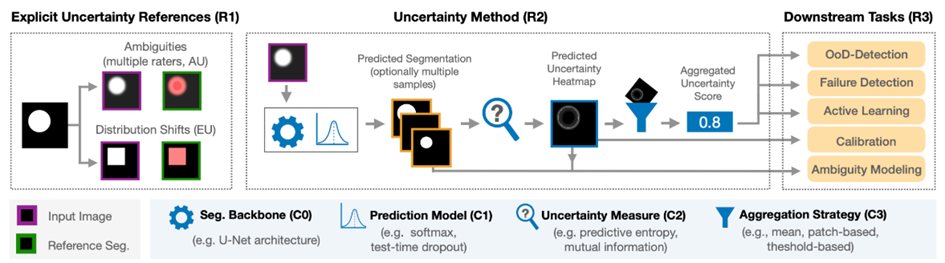
\includegraphics[width=\linewidth]{ValUES.png}
    \caption{Architecture ValUES}
    \label{fig:ValUES}
\end{figure}

Ce cadre est constitué de 3 parties : R1, R2 et R3.

\begin{itemize}
    \item \textbf{R1 :} Il évalue les méthodes d'incertitude prétendant séparer l'Incertitude Aléatoire et l'Incertitude Épistémique au moyen de références explicites, de métriques et de jeux de données de test.
    \item \textbf{R2 :} Il évalue les méthodes d'incertitude concernant tous les composants d'une méthode d'incertitude. Afin d'évaluer les capacités d'une méthode d'incertitude, il est crucial de retracer les améliorations à ses composants individuels C0, C1, C2 et C3.
    \begin{itemize}
        \item \textbf{C0 :} Appelé le backbone de segmentation, il s'agit de l'architecture utilisée pour la segmentation sémantique. Dans notre cas, nous utilisons l'architecture nnU-Net.
        \item \textbf{C1 :} Le modèle de prédiction est le modèle obtenu après l'entraînement des neurones de l'architecture sélectionnée.
        \item \textbf{C2 :} La mesure d'incertitude implique le calcul d'un score d'incertitude par voxel basé sur les scores de classe prédits, qui peuvent être représentés sous forme de carte thermique d'incertitude. Des exemples de mesures d'incertitude incluent l'Entropie Attendue et l'Information Mutuelle.
        \item \textbf{C3 :} La stratégie d'agrégation correspond à la stratégie utilisée pour agréger la carte thermique d'incertitude en une seule valeur scalaire au niveau de granularité souhaité en fonction de la tâche en aval. Cela permet aux cliniciens de passer de l'incertitude au niveau du voxel à l'incertitude au niveau de la lésion, par exemple. Comme nous nous intéressons à la quantification de l'incertitude appliquée aux voxels, nous ne considérerons pas cette partie.
    \end{itemize}
    \item \textbf{R3 :} Pour que les praticiens puissent décider si une méthode d'incertitude existante est adéquate pour leur tâche spécifique, il est crucial que les méthodes proposées soient généralement validées sur un large spectre de tâches en aval telles que : Bancs d'essai pour les 5 applications prédominantes de l'incertitude : Détection Hors Distribution (OoD-D), Apprentissage Actif (AL), Détection de Défaillance (FD), Calibration (CALIB), et Modélisation de l'Ambiguïté (AM). Plus d'informations sur ces métriques seront fournies ci-dessous.
\end{itemize}

\subsubsection{Quantification de l'incertitude inter-expert et défi CURVAS}

Le challenge \emph{CURVAS} (Calibration et Incertitude pour l'Évaluation de Volume Multi-Évaluateurs dans la Segmentation Multi-Organes), qui s'est tenu de mai à octobre 2024, a mis au défi des équipes de produire un modèle de segmentation qui détermine avec précision la meilleure calibration et quantification de la variabilité inter-experts. Nous utilisons le jeu de données fourni pour ce défi, qui contient un total de 90 scans CT de patients -- c'est-à-dire des images produites par un scanner à section transversale (CT) -- ainsi que 3 jeux d'annotations faites par 3 différents experts pour le pancréas, les reins et le foie(Voir La figure~\ref{figure:3d} pour le premier patient de la cohorte. Ces scans CT ont été obtenus à l'Hôpital Universitaire d'Erlangen entre août et octobre 2023. 20 scans CT ont été fournis pour l'entraînement (Groupe A), 5 pour la validation (Groupe A), et 65 pour les tests (20 dans le Groupe A, 22 dans le Groupe B, et 23 dans le Groupe C).). 

Dans le repository git CURVAS, plusieurs métriques peuvent être utilisées pour calculer l'incertitude générée par les annotations multi-évaluateurs.

    \begin{itemize}
        \item \textbf{Dice Similarity Coefficient ($DSC$) :}
        La première métrique que nous utiliserons est l'évaluation du Score de similarité de Dice (DSC), qui évaluera uniquement les zones de consensus de premier plan et d'arrière-plan pour trois classes : pancréas, rein et foie. Cela signifie que toute prédiction dans la zone de dissensus sera ignorée. Les Faux Positifs (FP) ne peuvent survenir que dans la zone de consensus d'arrière-plan, et les Faux Négatifs (FN) ne peuvent survenir que dans la zone de consensus de premier plan. Le DSC permet de quantifier le recouvrement spatial entre la prédiction et la réelle annotation (appelée "ground truth" ou "vérité terrain"). Cette métrique doit être haute.
    
        \begin{align*}
            \text{DSC} &= \frac{2 \times |\text{Prédiction} \cap \text{Vérité Terrain}|}{|\text{Prédiction}| + |\text{Vérité Terrain}|} \\
                      &= \frac{2TP}{2TP + FP + FN}
        \end{align*}
    
        \item \textbf{Confidence or Uncertainty assessement ($C_{seg}$):} De plus, nous prévoyons d'étudier l'incertitude au sein des régions de consensus. Cette étude sera divisée en deux parties : la confiance moyenne sera calculée séparément pour les zones de consensus d'arrière-plan ($C_B$) et de premier plan ($C_F$) de chaque classe (pancréas, rein et foie). Ensuite, nous moyennons la métrique de confiance par classe en considérant les deux régions de consensus pour obtenir $C_{seg}$. Cette métrique doit être haute.
        %
        \[ C_{\text{seg}} = \frac{(1 - C_B) + C_F}{2} \]
    
        \item \textbf{Expected Calibration Error (ECE) :}
        Cette métrique mesure la mauvaise calibration en comparant la précision et la confiance à travers différents bins de prédiction. Un bin, noté \( B_m \), est le groupe ou intervalle de confiance auquel appartient le voxel \( m \) (pixel en 3D) relativement à sa probabilité softmax donnée par le réseau de neurones. Chaque bin \( B_m \) contient \( |B_m| \) échantillons, avec \( acc(B_m) \) représentant la précision et \( conf(B_m) \) représentant la confiance. Avec \( n \) étant le nombre total d'échantillons, nous obtenons l'ECE comme suit. Cette quantité doit être faible.
        %
        \[
        \text{ECE} = \sum_{m=1}^{M} \frac{|B_m|}{n} \big| acc(B_m) - conf(B_m) \big|
        \]
    
        \item \textbf{Continous Ranked Probability Score (CRPS) :}
        Le Score de Probabilité Classée Continue est utilisé pour évaluer à quel point la distribution volumétrique prédite s'aligne avec la vérité terrain (précision). Pour conserver la variabilité multi-annotateurs, nous définissons une Fonction de Densité de Probabilité Gaussienne (PDF) basée sur la moyenne et l'écart-type des volumes dérivés des trois annotations d'experts. À partir de cela, nous calculons la Fonction de Distribution Cumulative (CDF) correspondante. La fonction de Heaviside, notée \(\bdOne_{\{x \geq y\}}\), est essentielle pour transformer la vérité terrain en une fonction indicatrice, permettant ainsi de comparer directement la CDF prédite à la réalité. Le volume prédit est obtenu en sommant toutes les valeurs probabilistes pour la classe correspondante à partir de la sortie probabiliste fournie par le participant. Cette approche intègre l'incertitude du modèle dans l'estimation du volume.
        %
        \[ \text{CRPS}(F, y) = \int \left( F(x) - \bdOne_{ \{x \geq y\}} \right)^2 \, dx \]
    
    \end{itemize}

    \refstepcounter{section}
    \label{cliguide}
    \addcontentsline{toc}{section}{\numberline{\thesection}{Guide d'utilisation de CLI}}
    \includepdf[pages=-,landscape=true]{Documentation CLI.pdf}

\end{document}